\documentclass[11pt]{exam}

\usepackage{amsmath} % allows for align environment
\usepackage{amssymb} % 
\usepackage{array} % for table alignments

% FONT FORMAT
% \renewcommand*\rmdefault{ppl} % change font to Palatino
\renewcommand*\rmdefault{lmss} % change font to lat mod ss

% ADJUST MARGINS
\usepackage[bmargin=1.0in]{geometry}
\geometry{margin=1in}
\geometry{tmargin=1in}

% TIKZ DIAGRAMS
\usepackage{tikz}
\usetikzlibrary{automata, arrows.meta}
\usetikzlibrary{arrows, automata} 
\usetikzlibrary{calc} 
\tikzset{
  vector/.style={thick, -{Stealth[length=5mm]}},
  }
% \usepackage{color}

  
\begin{document}

\begin{center}
    \Large MATH 1554 QH \\[2pt] Written Assignment 3
\end{center}
\thispagestyle{empty} % suppress page numbering

    Please \textbf{show your work} for each of the questions below.

\begin{questions}

    \question[5] Consider the matrix $A$ below, where $k$ is a real number.
    $$A=\begin{pmatrix} -2 & 2 & 2 \\ 2 & k & -1 \\ -6 & 3 & 5 \end{pmatrix}$$
    \begin{parts}
        \part Compute the determinant of $A$.
        \part Identify the values of $k$ for which the matrix $A$ is singular.
        \part Determine the eigenvalues of $A$ for the values of $k$ you identified in the previous part. \textit{Hint: you should not need to use polynomial division in this course. For this exercise, the third order polynomial can be simplified. }
        \part Construct the eigenbasis for each eigenvalue when $A$ is singular.
    \end{parts}

    \question[5] Consider the Markov chain below.
    \begin{center}
    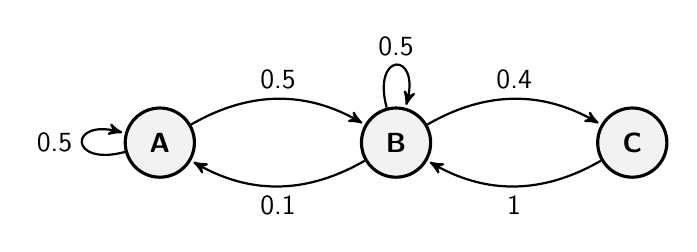
\begin{tikzpicture}[->,>=stealth',shorten >=1pt,auto,node distance=3cm,thick]
    \tikzstyle{every state}=[circle,fill=gray!10,draw,thick,font=\bf, line width=0.4mm]

    \node[state] (A) {A};
    \node[state]  (C) [right of=A] {B};
    \node[state]  (B) [right of=C] {C};    
    \path 
        (A) %edge [bend left] node {0.2} (B)
            edge [loop left] node {0.5} (A)
            edge [bend left] node {0.5} (C)
        (B) %edge [bend left] node {0.4} (A)
            %edge [loop right] node {0.4} (B)
            edge [bend left] node {1} (C) 
        (C) edge [bend left] node {0.1} (A)
            edge [bend left] node {0.4} (B)
            edge [loop above] node {0.5} (C); 
    \end{tikzpicture} 
    \end{center}    
    \begin{parts} 
        \part Identify the transition matrix, $P$, for the Markov chain.
        \part Determine whether the Markov chain is regular.
        \part Calculate the steady state for the Markov chain.     
    \end{parts}

\noindent Please ensure that you follow the instructions below. 
\begin{itemize}
    \item Your work is legible in the files you uploaded. 
    \item Questions are answered in the order in which they were given. 
    \item During the upload process, you indicated which pages correspond to which question.
    \item During the upload process that none of your pages are upside down or sideways. 
    \item Each question is answered on its own page (or pages). 
    \item Your work is submitted as a single PDF file.
    \item You uploaded your work to the correct location in Gradescope (in other words, make sure that you upload your work for this assignment to the correct assignment).
\end{itemize}
\noindent Note that
\begin{itemize}
    \item A small amount of points (at most 1 point) will be deducted from the assignment for not following the instructions listed above. 
    \item You can also change the orientation of the pages when you upload in Gradescope. 
    \item Ensuring that these criteria are met helps ensure that your work is graded efficiently and accurately. 
\end{itemize}
    
    
\end{questions}

\end{document}
